\documentclass[10pt,letterpaper]{article}
\usepackage[margin=0.65in]{geometry}
\usepackage{graphicx}
\usepackage{amsmath}
\usepackage[colorlinks=true,allcolors=blue]{hyperref}
\title{CRF-SAM3: Supplementary Material}
\author{Anonymous Submission}
\date{}
\begin{document}
\maketitle
\section*{Training labels and candidate caches}
\paragraph{Category targets for the grounder.} The concept loss $\mathcal{L}_{\mathrm{cat}}$ requires a category label $c^{\star}$ for each training expression. On Ref-Youtube-VOS, $c^{\star}$ is the annotated object category. ReVOS does not provide object categories, so for its training split we query Qwen3.7-Plus once per expression with the complete referring expression and up to three temporally ordered training frames on which the ground-truth target box is drawn, and ask for a single JSON field \texttt{category}. The returned names are normalized before training. Because these boxes are derived from ground-truth masks, the labels are used only as training targets; they are never computed for validation or test videos and are not used by any reported inference run.

\paragraph{Concepts for the verifier training caches.} Verifier training candidates are generated offline with the same SAM3 recall procedure as at inference ($K_r=24$, $K_{\mathrm{keep}}=7$). For MeViS, Ref-DAVIS17, and Ref-Youtube-VOS, the cache is prompted with concepts produced by a prompt-based Qwen3-VL concept extractor on the training videos; for ReVOS, it is prompted with the category labels above. Candidates are then labelled by their sequence-level IoU with the ground-truth tube (main paper, Sec.~3.3). Since the verifier consumes only candidate tubes and the expression, its training does not depend on the grounder.

\clearpage
\section*{Real qualitative evidence}
\noindent All examples use the completed ReVOS validation run. Historical predictions and scores are kept separate from a frozen-SAM3 recall replay performed for visualization. Each selected replay tube matches the historical prediction pixel-for-pixel over the complete sequence. This does not certify the unarchived historical masks of unselected candidates. Reported J\&F values are full-sequence metrics. Case selection is diagnostic and illustrative, not statistical sampling.
\begin{figure}[h]
\centering
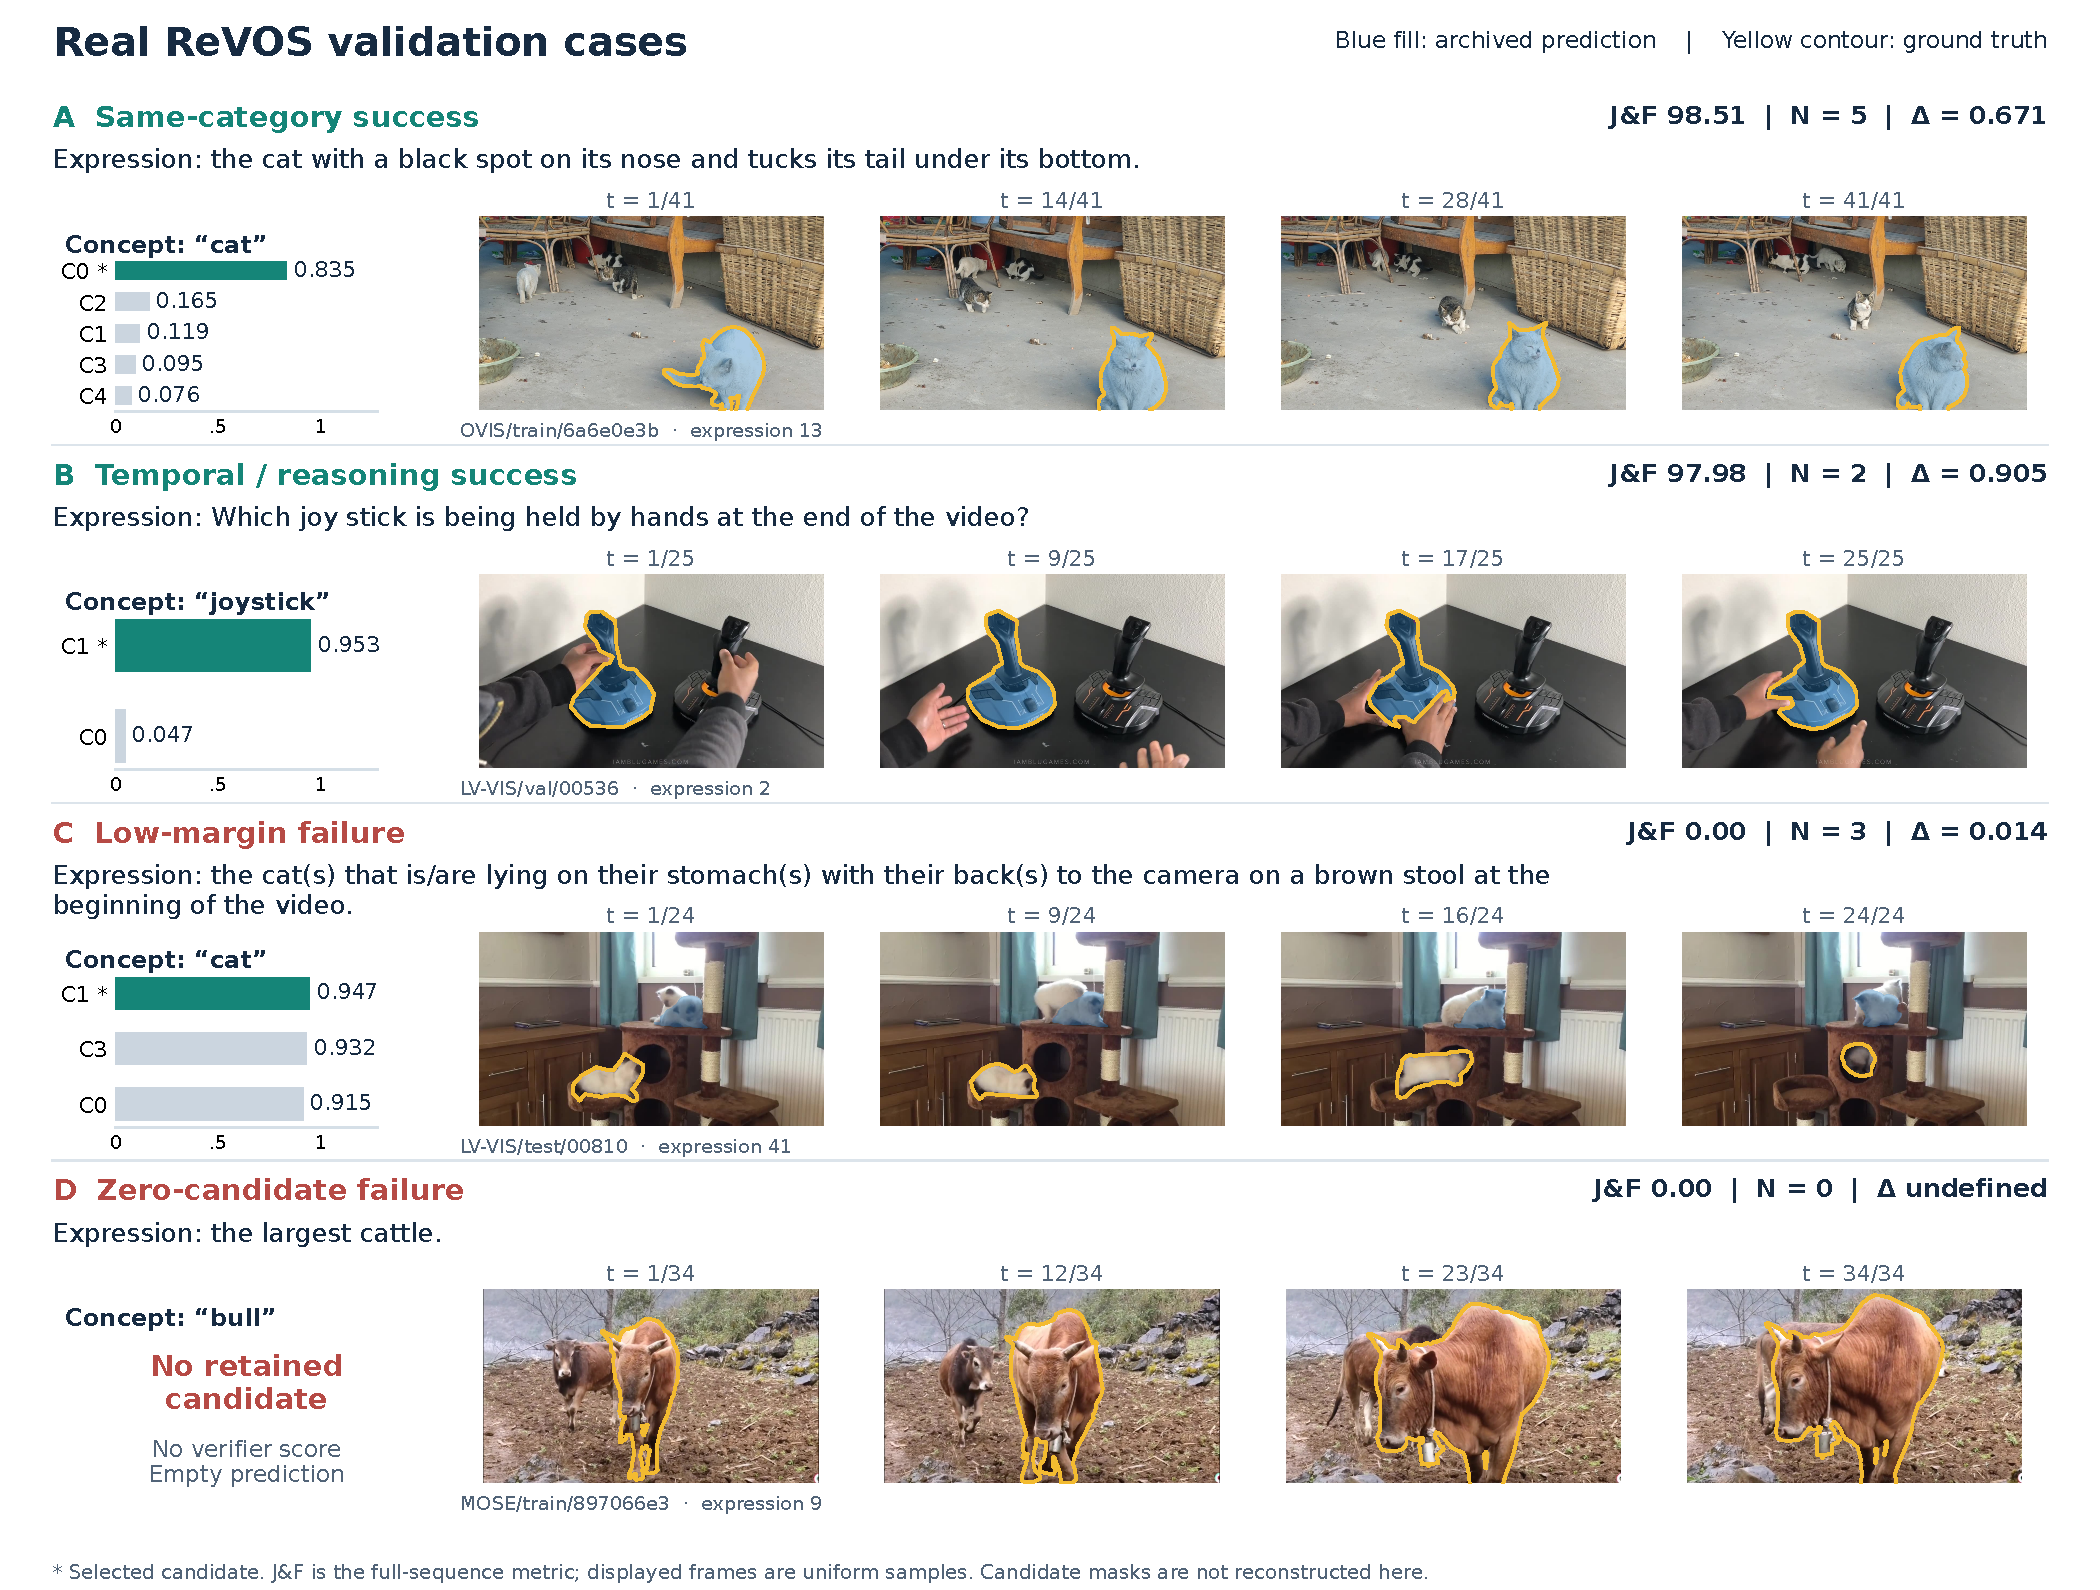
\includegraphics[width=\textwidth]{figures/revos_qualitative_archived.pdf}
\caption{Four uniformly sampled time steps per case. Blue fill shows the archived prediction; yellow contours show GT. No replay masks are used in this plate. The visible source paths are constituent dataset identifiers within the ReVOS validation split.}
\end{figure}
\clearpage
\section*{Case A: same-category candidate set}
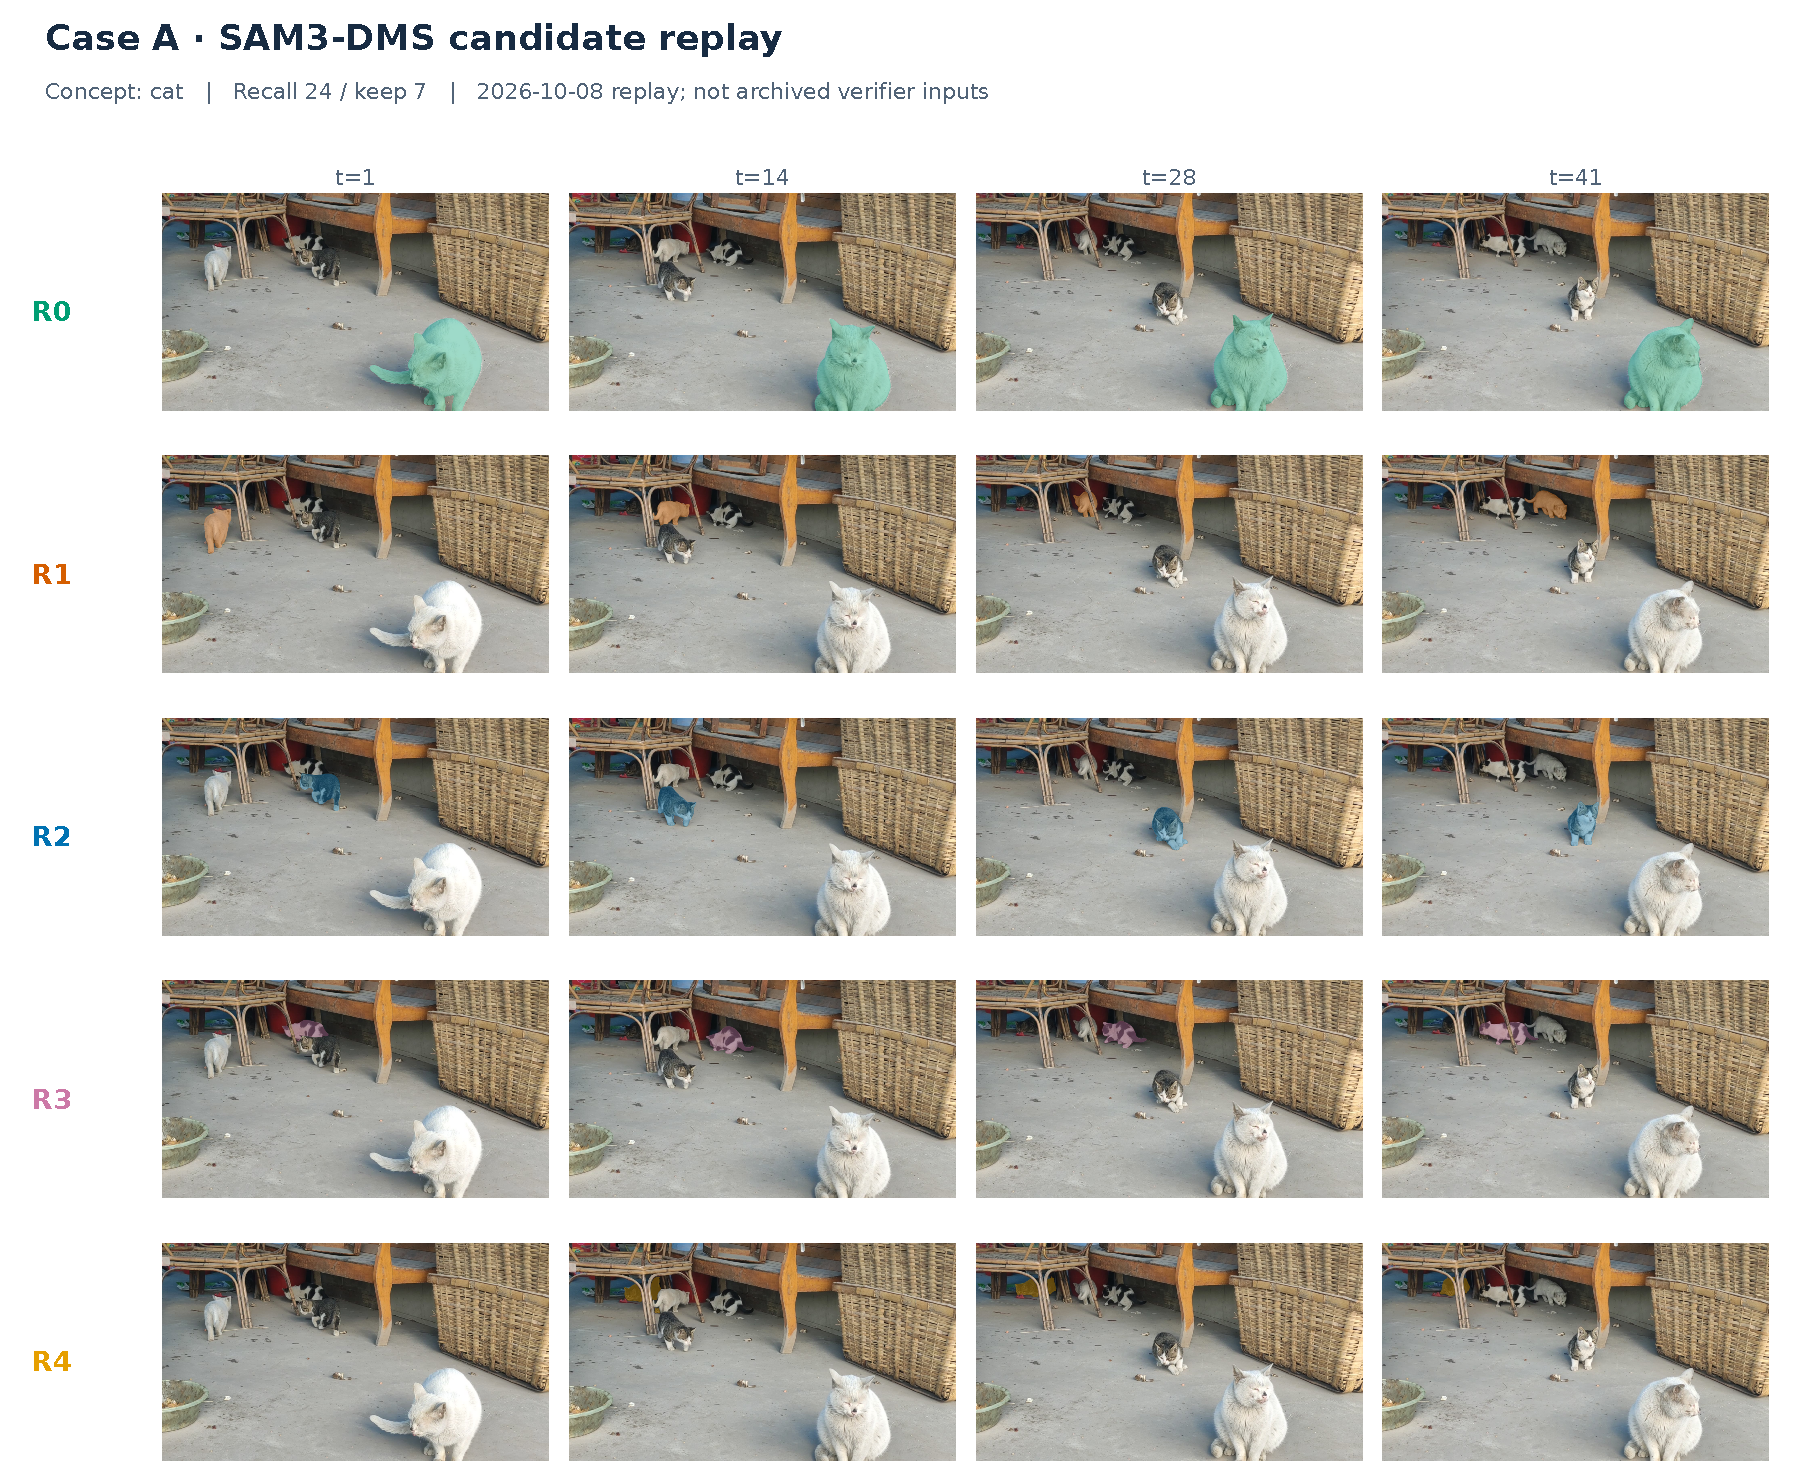
\includegraphics[width=\textwidth,height=0.86\textheight,keepaspectratio]{figures/case_A_candidate_replay.pdf}
\clearpage
\section*{Case B: temporal expression}
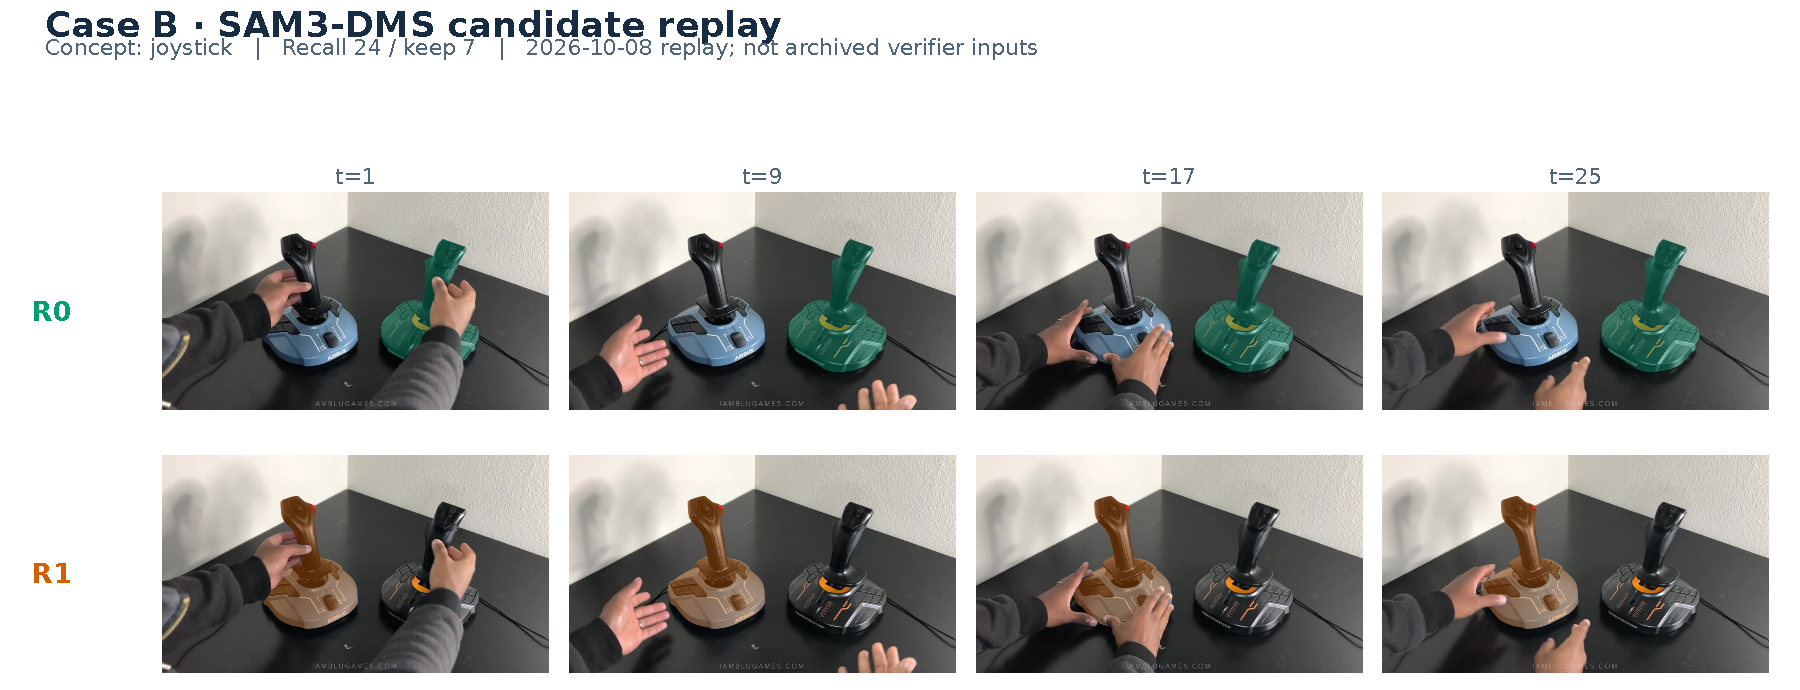
\includegraphics[width=\textwidth]{figures/case_B_candidate_replay.pdf}
\noindent Replayed R1 matches the archived selected C1 in all 25 frames; recorded probabilities are 0.953 for C1 and 0.047 for C0. The original expression is ``Which joy stick is being held by hands at the end of the video?''
\clearpage
\section*{Case C: low-margin error}
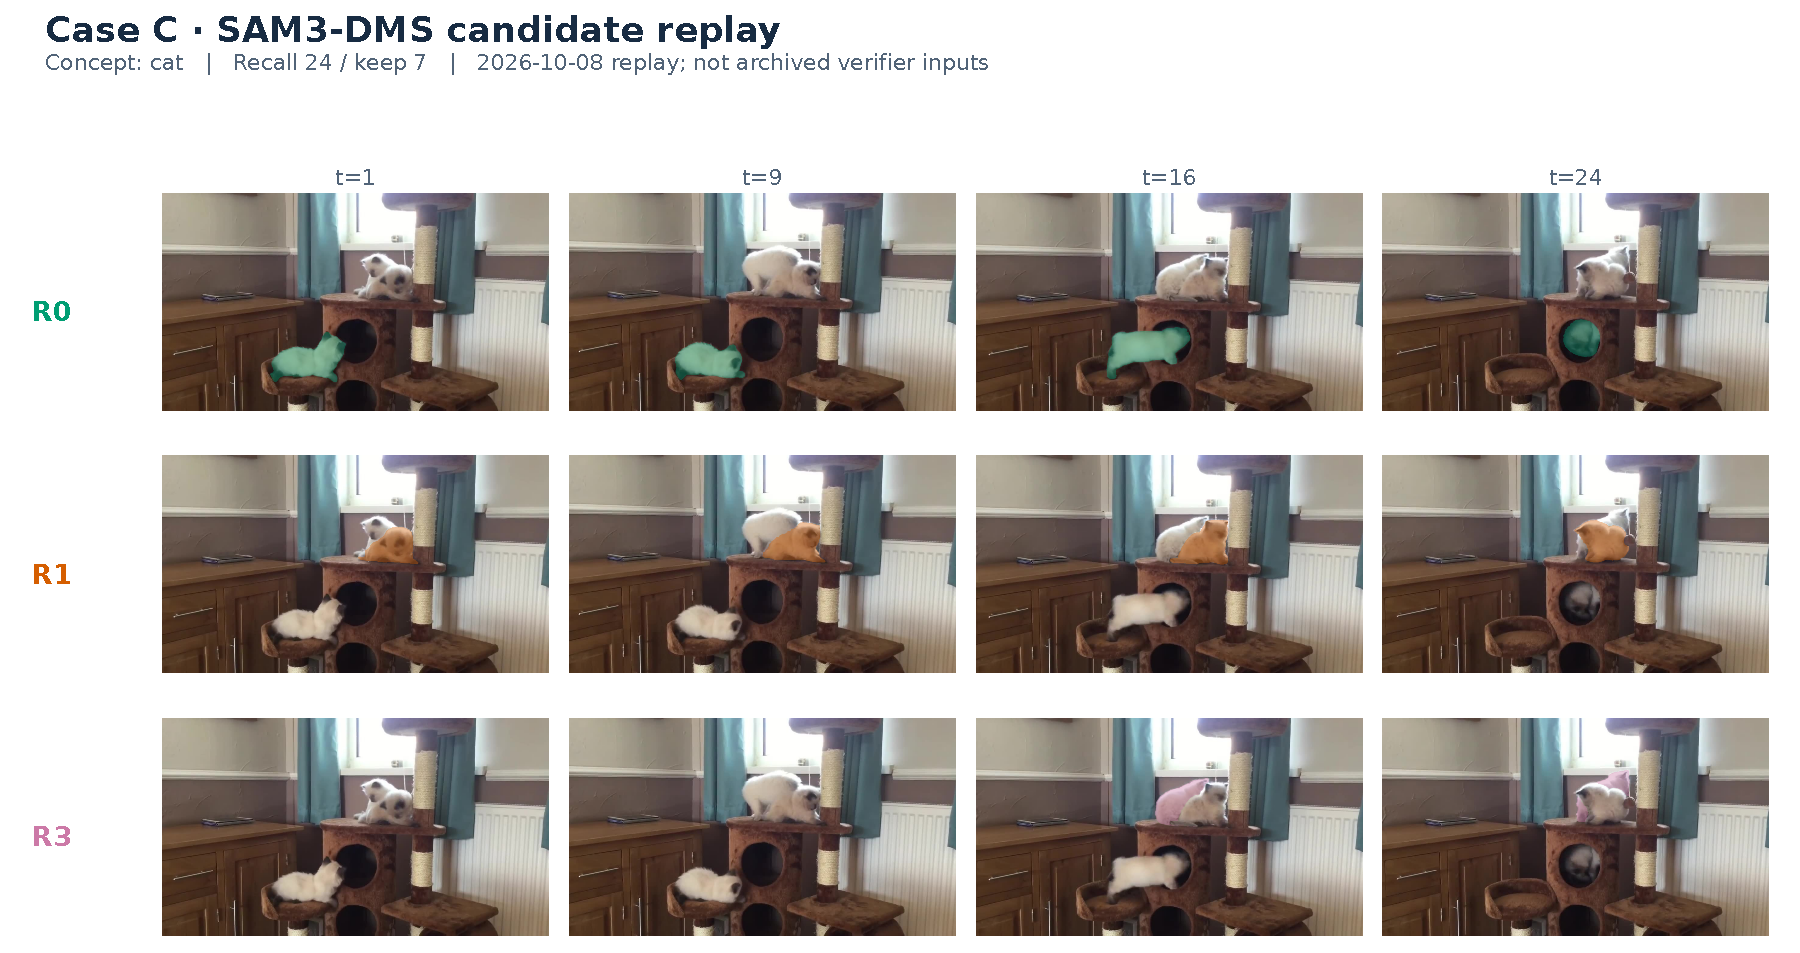
\includegraphics[width=\textwidth]{figures/case_C_candidate_replay.pdf}
\noindent The archived scores are C1: 0.947, C3: 0.932, C0: 0.915. The replayed R1 matches the archived selected C1 in all 24 frames and has J\&F=0. Replayed R0 has J\&F=93.86 against GT. Candidate IDs and cardinality agree, but the historical unselected masks were not retained; the alternative-mask metric is explicitly a replay diagnostic.
\end{document}
